%-----General Settings----%
\documentclass{other/docTemplate}
\svnid{$Id$}

\author{ML: Gonzalo Ducca \formatemail{gonzaloducca@gmail.com} \\ DA: Juan P. Bertone \formatemail{bertonejpb@gmail.com} \\ DE: Juan E. Flórez-Coronel \formatemail{juan.florez@upr.edu} \\ DA: Valentino Caputa \formatemail{caputavalentino@gmail.com} \\ ML: Carlos Madoery \formatemail{ccmadoery@gmail.com}}  
\po{Melina Griffo \formatemail{meligriffo@gmail.com}}
\title{Reporte del Proyecto Fianl: Expectativa de vida al nacer} 
\henrymentor{Pía Ruiz \formatemail{mpiaruiz@gmail.com}}

\loadglsentries{other/acronyms}
\makeglossaries

%-----Beginning of Document----%
\begin{document} 
\maketitle

%---Revision Tracker---%
\startTable
\AddRevision{0.0}{10-20-23}{Creación del documento}
\AddRevision{1.0}{11-01-23}{Documentación Sprint 1}
\AddRevision{2.0}{11-15-23}{Documentación Sprint 2}
\stopTable

%-----Table of Contents-----%
\tabladecontenido
\newpage
\listadetablas
\newpage
\listadefiguras
\newpage
\printglossary[title=Lista de Acronimos ,type=\acronymtype]
\clearpage

%-----Acknowledgments-----%
%\section*{Acknowledgments}
%\addcontentsline{toc}{section}{Acknowledgments}%adds acknowledgements section to the table of contents

%Here is a sample for how to susse acronyms. "Defining a \gls{fr} and a \gls{ps} provides a language for system design. This language is an important aspect of \gls{csd}."
%\newpage

%-----Abstract-----%
%\section*{Abstract}
%\addcontentsline{toc}{section}{Abstract}%adds Abstract section to the table of contents
%\newpage

%-----Content-----%
%%%%%%   PLANTEAMIENTO DEL PROBLEMA  %%%%%%                                               
\section{Planteamiento del problema}
Consultamos bases de datos del Banco Mundial y decidimos utilizar como referencia temas clave que proporcionan indicadores que influyen en la esperanza de vida de los habitantes de un país. Estos temas seleccionados son la educación, la salud, la economía, el desarrollo de la ciencia y la tecnología y el ámbito social.
Planeamos recopilar indicadores de cada tema, crear las bases de datos con las que queremos trabajar y luego vincular estas variables para establecer relaciones. Visualizamos este proyecto como un producto que se puede ofrecer a una empresa que busque invertir en ciencia y desarrollo.
Una vez completado todo el trabajo de análisis de datos, crearemos modelos de aprendizaje automático especificando ciertos parámetros, como el porcentaje del \gls{pib} invertido en educación o ciencia. Estos modelos luego nos proporcionarán una esperanza de vida estimada para un país en particular.

%%%%%%  PLANTEAMIAENTO DEL PROBLEMA - Objetivos  %%%%%% 
\subsection{Objetivos}
Analizar la expectativa de vida en 30 paises en base a 5 factores:
\begin{itemize}
  \item Educación
  \item Salud
  \item Economía
  \item Ciencia y Tecnología
  \item Social
\end{itemize}

%%%%%%  PLANTEAMIENTO DEL PROBLEMA - Público objetivo  %%%%%% 
\subsection{Público objetivo}
El público obejtivo de este proyecto incluye entidades públicas y privadas con intereses creados en el tema y usuarios cotidianos que quieran conocer la esperanza de vida esperada en un país determinado. 
 Las instituciones públicas, como las agencias gubernamentales, pueden utilizar los conocimientos y modelos generados para informar decisiones políticas y asignar recursos de manera efectiva en áreas relacionadas con la educación, la atención médica y la investigación científica. Por otro lado, las empresas privadas, especialmente aquellas involucradas en industrias relacionadas con la ciencia y la tecnología, pueden beneficiarse de los hallazgos del proyecto al tomar decisiones de inversión e iniciativas de responsabilidad social corporativa. Este proyecto está dirigido a una amplia gama de organizaciones que buscan tomar decisiones informadas que impacten el bienestar y el desarrollo de los países.

%%%%%%   PLANTEAMIENTO DEL PROBLEMA - Alcance del proyecto %%%%%%  
\subsection{Alcance del proyecto}
El alcance del proyecto implica un análisis exhaustivo de la esperanza de vida en 30 países de todo el mundo durante los últimos 35 años. Este análisis abarcará cinco temas clave dentro de cada uno de los cinco factores influyentes, a saber, educación, salud, economía, ciencia y tecnología y ámbito social. El objetivo es proporcionar una visión detallada y basada en datos de los factores que afectan la esperanza de vida en estos países durante el período de tiempo especificado.
 El producto final incluirá un servicio web donde se pueda acceder a la información brindada por el análisis y un dashboard interactivo con insights claves para la interpretación de los datos. 


%%%%%%  Obtención de los datos %%%%%%  
\clearpage
\section{Obtención de los datos}
La información fue obtenida utilizando la siguiente API \href{https://datahelpdesk.worldbank.org/knowledgebase/topics/125589}{World Bank API}.

%%%%%%   API %%%%%%  

\subsection{World Bank API}

La información de la API de World Bank tiene los siguientes tópicos:

\begin{figure}[htbp!]
  \centering
  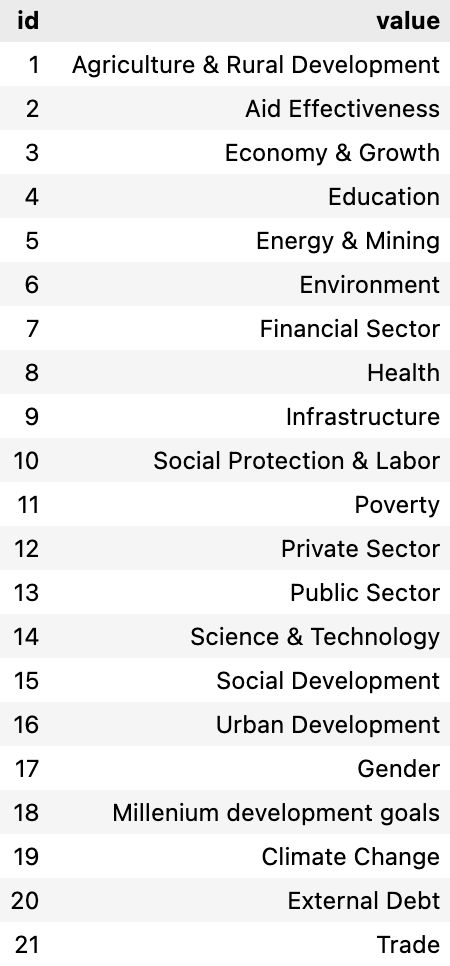
\includegraphics[width=0.4\textwidth]{topics.png}
  \caption{Tópicos World Bank}
  \label{fig:topics}
\end{figure}

Y las siguientes economías:

\begin{figure}[htbp!]
  \centering
  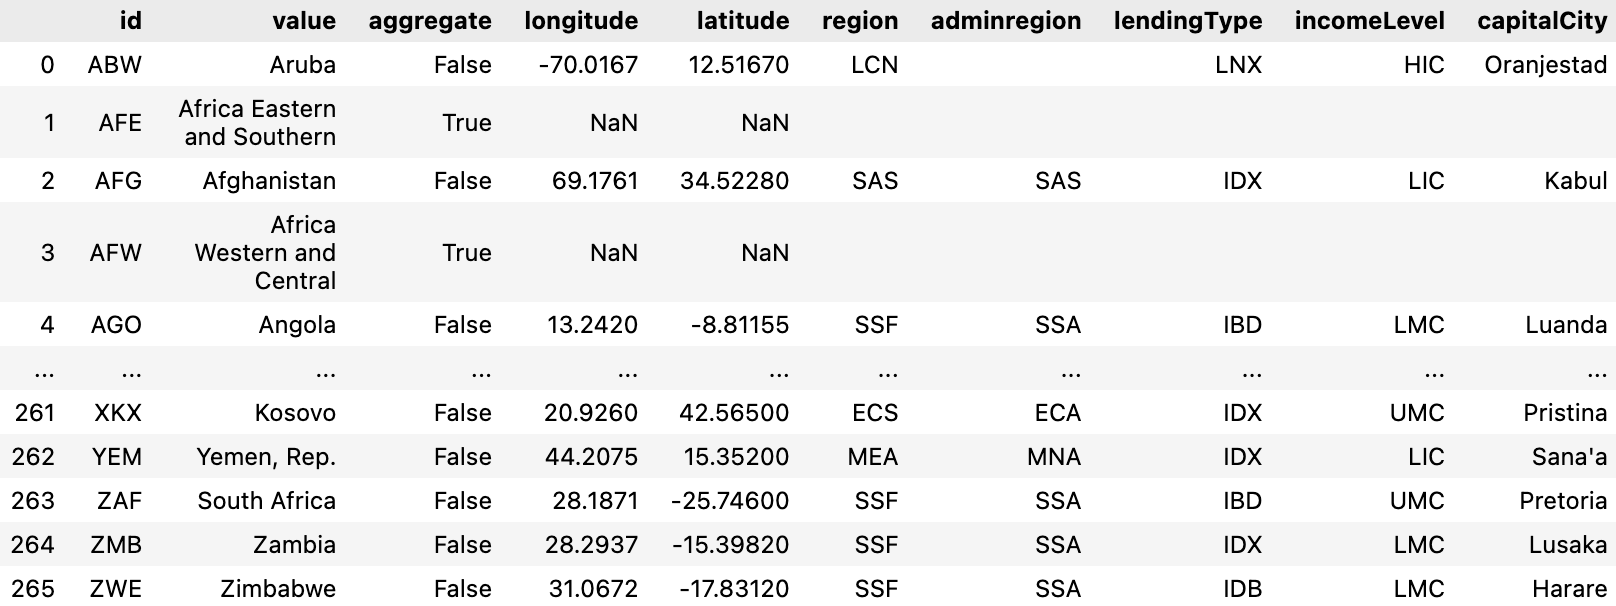
\includegraphics[width=0.9\textwidth]{economies.png}
  \caption{Economías World Bank}
  \label{fig:economies}
\end{figure}

Cada tópico tiene factores asociados:

\begin{figure}[htbp!]
  \centering
  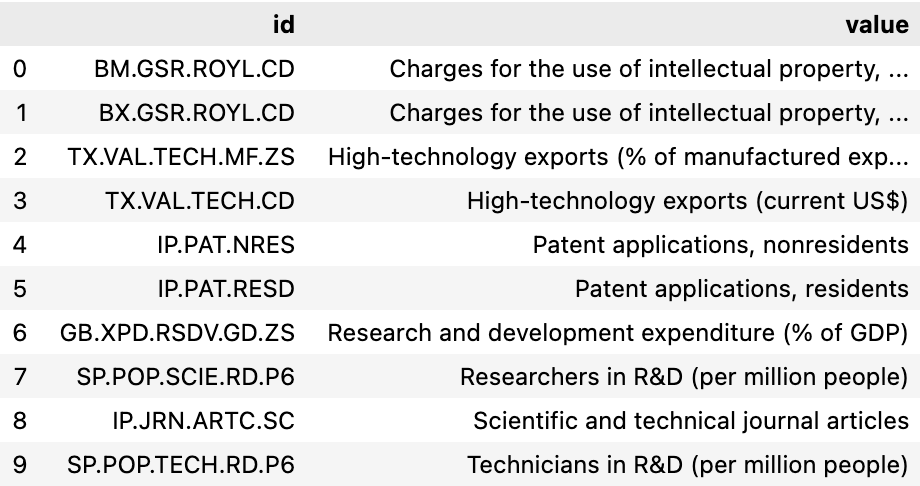
\includegraphics[width=0.7\textwidth]{st_factors.png}
  \caption{Factores Ciencia y Tecnología World Bank}
  \label{fig:stfactors}
\end{figure}

%%%%%%   Tópicos Posibles %%%%%% 

\subsection{Tópicos Posibles}

Contando valores faltantes:

\begin{figure}[htbp!]
  \centering
  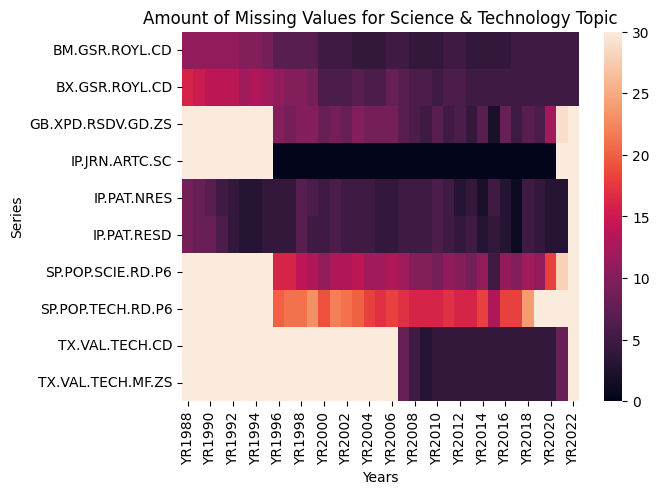
\includegraphics[width=0.7\textwidth]{Nan.png}
  \caption{Análisis de valores Nan}
  \label{fig:nan}
\end{figure}

\clearpage
\section{Desarrollo del Proyecto} 
\subsection{Roles del Equipo}
\begin{table}[H]
  \centering	
  \caption{Roles del Equipo}
  \begin{tabular}{|p{5cm}|p{10cm}|}
    \hline
    \textbf{Role} & \textbf{Name} \\\hline
    Machine Learning & Gonzalo Ducca \\\hline
    Machine Learning & Carlos Madoery \\\hline
    Data Analytics & Valentino Caputa \\\hline
    Data Analytics & Juan P. Bertone \\\hline
    Data Engineer & Juan E. Flórez-Coronel \\\hline
  \end{tabular}
  \label{tab:teamroles}
\end{table}
\subsection{Diagrama de Gaant}
\begin{figure}[htbp!]
  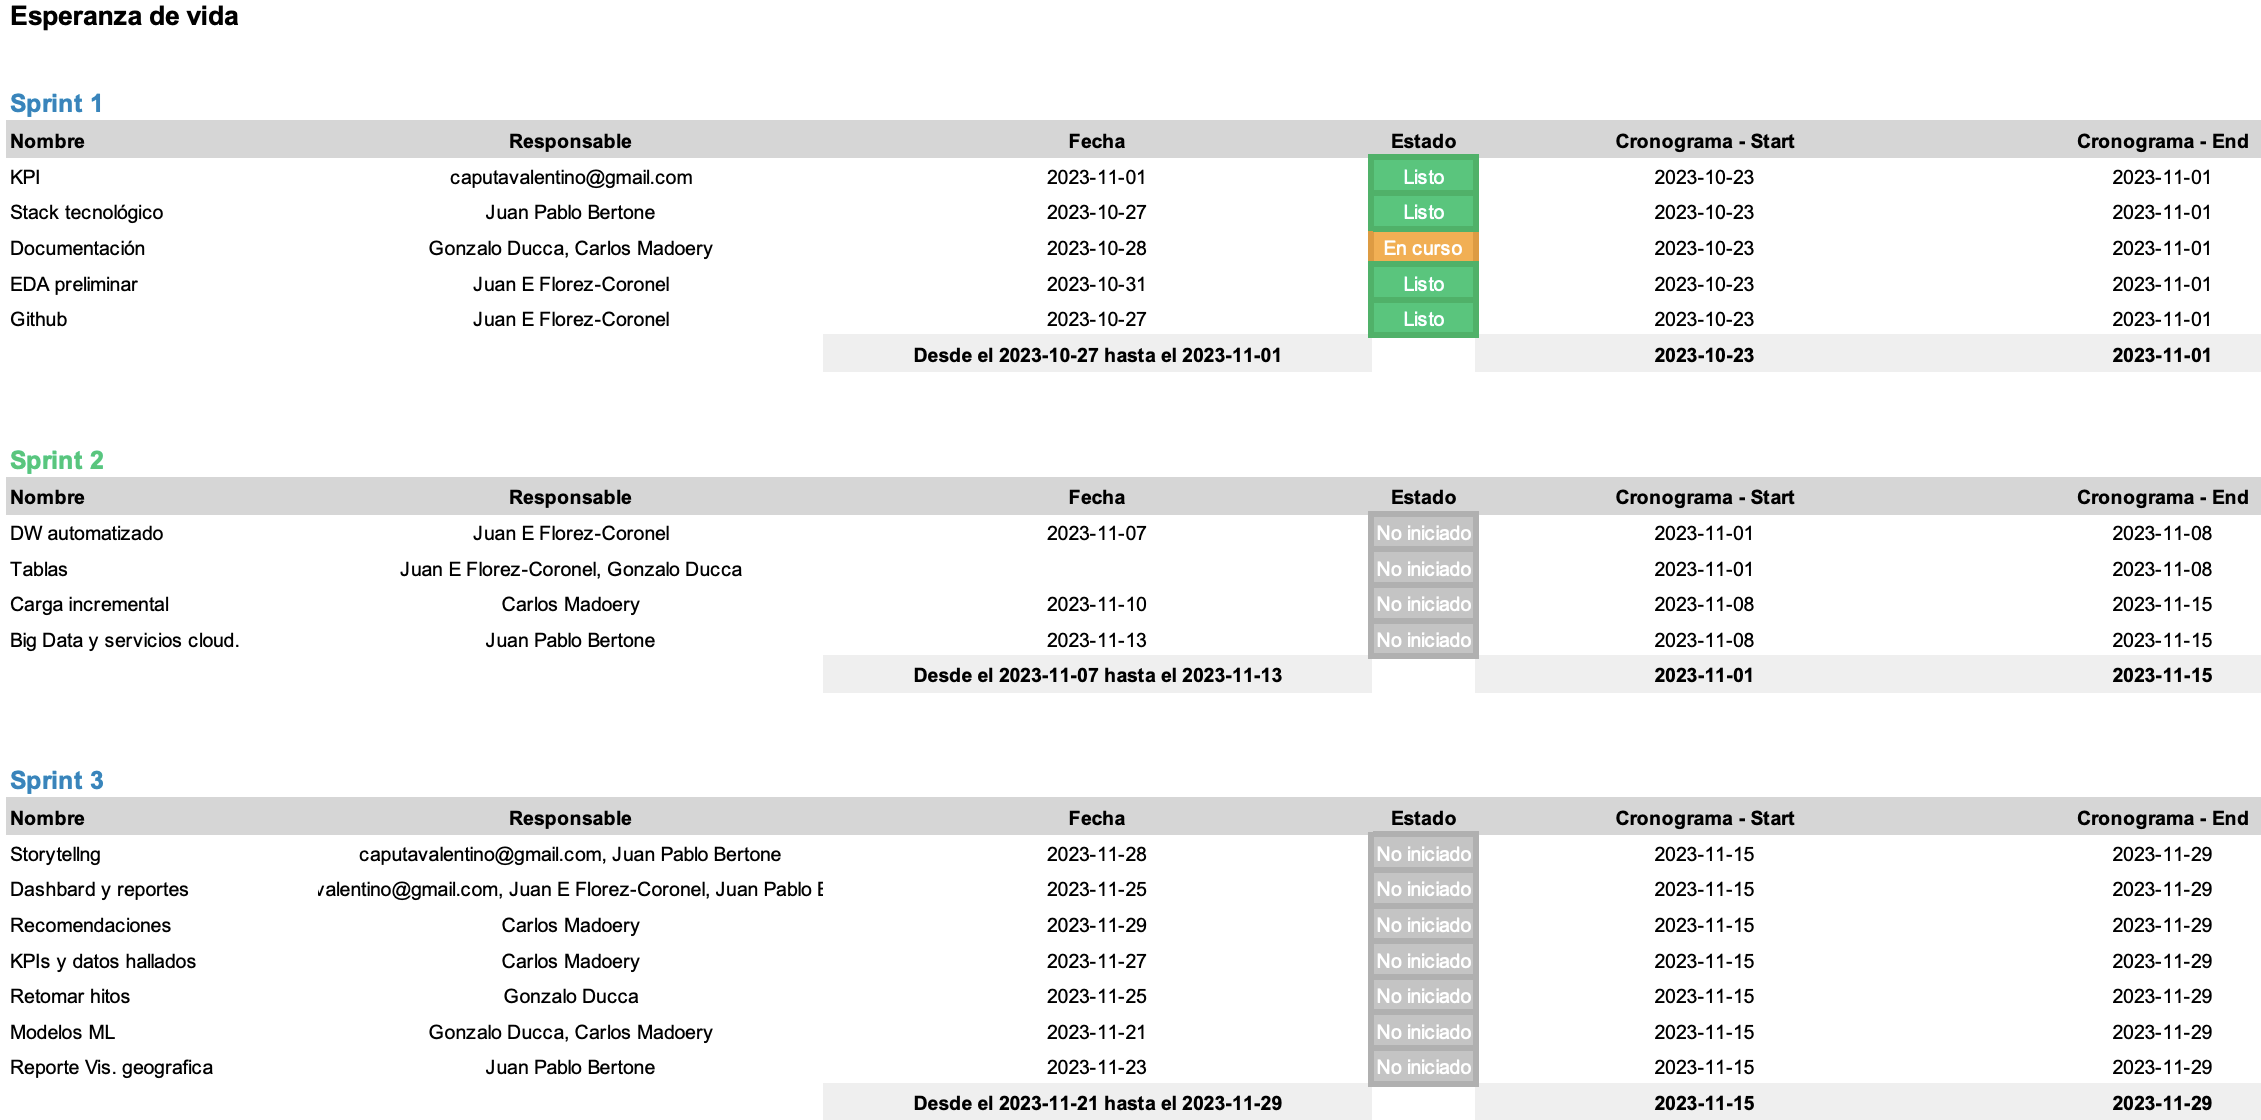
\includegraphics[width=\textwidth]{gaant.png}
  \caption{Diagrama de Gantt}
  \label{fig:gaant}
\end{figure}

%%%%%%   Conclusiones  %%%%%%  
\clearpage
\section*{Cconclusiones y Lecciones Aprendidas}
\addcontentsline{toc}{section}{Conclusiones y Lecciones Aprendidas}%adds Conclusions and Lessons Learned section to the table of contents

bla

%----References-----%
%\clearpage
%Please refer to the OverLeaf Primer to see your options for how to keep track of references.
%\section*{References}
%\addcontentsline{toc}{section}{References}%adds reference section to the table of contents
%Use the OverLeaf Primer to understand the different ways to format the references. 
%\bibliographystyle{IEEEtran} %Formats the bibliography to meet the IEEE standards
%\bibliography{ref.bib} %This command calls a file named "your_references.bib". You will upload this file, and can rename as necessary. 
  

%\clearpage
%\appendix
% \renewcommand{\thesection}{\Alph{section}.}
%\setcounter{section}{0}

%\addcontentsline{toc}{section}{Appendices}
%--Product System Design Decomposition----% 
%\section{Product System Design Decomposition}
%Provide a complete design decomposition. If the different branches relate to different parts of the product design (i.e safety, electrical subsystem, mechanical subsystem, etc...), please label those to show at a high level an overview of your decomposition. 

%Uncomment and use the below commands to include your decomposition. The "angle=90" rotates the decomposition to a landscape view. 

%-----------Figure------------%
% \begin{figure}[ht!]
% \centering
% \includegraphics[width=1.1\textwidth, angle=90]{Design_Decomposition}
% \caption{System Design Map}
% \label{System Design Map}
% \end{figure}
%-------End of Figure---------%


%--Design Drawings/Schematics----% 
%\clearpage
%\section{Design Drawings/Schematics}
%Please provide necessary drawings and schematics here. These should include both the mechanical and electrical figures if applicable. 


%----Appendix Proof of Material Purchase---% 
%\clearpage
%\section{Proof of Material Purchases}
%Please provide a copy of your receipt(s) for the purchase of the items on your bill of materials. 

%----Appendix: Other---% 
%\clearpage
%\section{Other}

\end{document}
